\documentclass[svgnames]{beamer}
\mode<presentation>
\usefonttheme{serif}
\usecolortheme{dove}
\useinnertheme{rounded}
\setbeamercolor{item projected}{fg=black}
\setbeamertemplate{navigation symbols}{}

\usepackage[english]{babel}
\usepackage[latin1]{inputenc}
\usepackage{times}
\usepackage{amsmath}
\usepackage{amsfonts}
\usepackage{amssymb}
\usepackage{amsthm}
\usepackage{graphics}
\usepackage{multicol}
\usepackage{framed}
\usepackage{ulem}
\usepackage{ifthen}
\usepackage{tikz}
\usepackage{gastex}
\usepackage{ulem}
\usepackage{booktabs}

\newcommand{\buc}{\mathrm{B\ddot{u}chi}}
\newcommand{\bucf}{\buc(F)}
\newcommand{\bucfn}{\buc(F,N)}

\newcommand{\fin}{\mathrm{Fin}}
\newcommand{\bnd}{\mathrm{Bnd}}
\newcommand{\co}{\mathrm{Co}}

\newtheorem{conjecture}{Conjecture}

\newcommand{\set}[1]{\{ #1 \}}
\newcommand{\push}{\mathrm{push}}
\newcommand{\pop}{\mathrm{pop}}
\newcommand{\Skip}{\mathrm{skip}}

\newcommand{\parp}{\mathrm{Parity}}
\newcommand{\bound}{\mathrm{Bound}}

\newcommand{\W}{\mathcal{W}}
\newcommand{\WE}{\W_{E}}

\newtheorem{observation}{Observation}
\newtheorem{proposition}{Proposition}

\renewcommand{\ULthickness}{1.2pt}

%%%%%%%%%%%%%%%%%%%%%%%%%%%%%%%%%%%%%%%%%%%%%%%%%%%%%%%%%%%%%%%%%%%%%%%%%%%%%%%
%%%%%%%%%%%%%%%%%%%% A non-original creation by Nathana�l Fijalkow and myself %

\setbeamertemplate{frametitle}{%
  \vskip-2pt%
  \begin{beamercolorbox}[rightskip=2cm,leftskip=1em,dp=1ex,wd=12.8cm]{frametitle}%
    \vskip2pt%
    \usebeamercolor{frametitle}%
    \begin{tikzpicture}[scale=1]%
      \useasboundingbox (0,0) rectangle (0,0); %(-1,-1) rectangle (1,1);%
      \ifthenelse{\insertframenumber<\inserttotalframenumber}%
      { % uncomplete tart

        \pgfmathsetmacro{\aimangle}{90-(\insertframenumber*360/\inserttotalframenumber)}
        \fill [fill=frametitle.fg,thin, color=gray!50,draw=black] (11.8,.2) -- (11.8,.6) arc (90:\aimangle:0.4) -- cycle;%

      }{ % the full tart
        \fill[fill=frametitle.fg,thin, color=gray!50,draw=black] (11.8,0.2) circle (.4);%
      }%
      \fill[fill=frametitle.fg,thin, color=white,draw=black] (11.8,0.2) circle (.3);%
      \node at (11.8, .2) [black,circle]{\normalsize\insertframenumber};

    \end{tikzpicture}
    \insertframetitle%
    \vskip2pt%
  \end{beamercolorbox}%
}
%%%%%%%%%%%%%%%%%%%%%%%%%%%%%%%%%%%%%%%%%%%%%%%%%%%%%%%%%%%%%%%%%%%%%%%%%%%%%%%


\setbeamertemplate{blocks}[rounded]%
\setbeamercolor{block title}{bg=normal text.bg!90!black}
\setbeamercolor{block body}{bg=normal text.bg!95!black}

\AtBeginSection[]
{
\addtocounter{framenumber}{-1}
  \begin{frame}<beamer>{Outline}
    \tableofcontents[currentsection]
  \end{frame}
}

\AtBeginSubsection[]
{
\addtocounter{framenumber}{-1}
  \begin{frame}<beamer>{Outline}
    \tableofcontents[currentsection,currentsubsection]
  \end{frame}
}

\begin{document}

\addtocounter{framenumber}{-1}

\title{Infinite-state games with finitary conditions}
\subtitle{CSL, September 5th, 2013}
\author{Krishnendu Chatterjee \and \underline{Nathana\"el Fijalkow}}
\institute{Institute of Informatics, Warsaw University -- Poland 
\and LIAFA, Universit\'e Paris 7 Denis Diderot -- France}
\date{}

\begin{frame}
\maketitle
\end{frame}

\begin{frame}{In a nutshell}
This paper is about $\omega B$-games, and the subclass of finitary games. 
\vskip1em
They are:
\begin{itemize}
\pause	\item two-player turn-based games played over \textbf{infinite} graphs,
\pause	\item the winning conditions involve counters,
\pause	\item the first issue is to prove the existence of finite-memory strategies,
\pause	\item the second issue is to construct algorithms to decide the winner.
\end{itemize}
\end{frame}

\begin{frame}{Motivation: expressing boundedness properties}
\begin{figure}[ht]
\begin{minipage}[b]{0.45\linewidth}
\centering
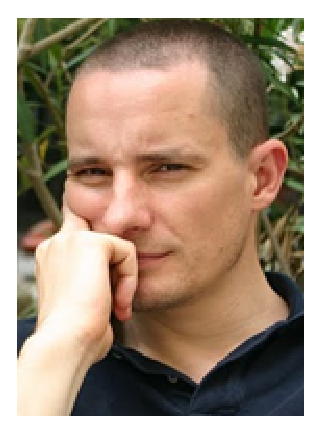
\includegraphics[width=19mm]{mikolaj}

$\mathrm{MSO} + \mathbb{U}$
\end{minipage}
\hspace{0.5cm}
\begin{minipage}[b]{0.45\linewidth}
\centering
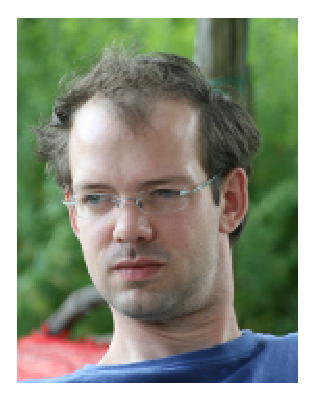
\includegraphics[width=20mm]{thomas}

$\mathrm{cost}\ \mathrm{MSO}$
\end{minipage}
\end{figure}
\begin{center}
A lot is known, and even more is not known about those two logics!
\end{center}
\end{frame}

\begin{frame}{Definition of $\omega B$-games}
\begin{center}
\begin{multicols}{2}
\begin{picture}(40,60)(0,0)
	\gasset{Nw=8,Nh=8}
	
  	\rpnode[polyangle=45](1)(30,15)(4,5){}
  	\node(2)(20,30){}
  	\node(3)(40,30){}
  	\rpnode[Nmarks=i,iangle=180,polyangle=45](4)(0,30)(4,5){}
  	\rpnode[polyangle=45](5)(10,50)(4,5){}
  	\node(6)(10,10){}
  	\rpnode[polyangle=45](7)(30,50)(4,5){}

  	\drawedge(1,2){}
  	\drawedge[curvedepth=3](1,3){}
	\drawloop[loopangle=90](2){}
  	\drawedge(2,3){}
  	\drawedge(2,6){}
  	\drawedge[curvedepth=5](3,1){}
  	\drawedge(4,2){}
  	\drawedge[curvedepth=5](4,5){}
  	\drawedge[curvedepth=5](5,4){}
	\drawloop[loopangle=-90](6){}
  	\drawedge(7,5){}

\only<8,15>{
  	\rpnode[polyangle=45](1b)(30,15)(4,5){{\color{red}{$1$}}}
  	\node(2b)(20,30){{\color{blue}{$2$}}}
  	\node(3b)(40,30){{\color{red}{$3$}}}
  	\rpnode[Nmarks=i,iangle=180,polyangle=45](4b)(0,30)(4,5){{\color{red}{$3$}}}
  	\rpnode[polyangle=45](5b)(10,50)(4,5){{\color{blue}{$2$}}}
  	\node(6b)(10,10){{\color{blue}{$4$}}}
  	\rpnode[polyangle=45](7b)(30,50)(4,5){{\color{blue}{$0$}}}
}

\only<9,10,11,12,13,14,15>{
  	\drawedge(1,2){$i,\varepsilon$}
  	\drawedge[curvedepth=3](1,3){$\varepsilon,i$}
	\drawloop[loopangle=90](2){$i,i$}
  	\drawedge(2,3){$\varepsilon,\varepsilon$}
  	\drawedge[ELside=r](2,6){$i,r$}
  	\drawedge[curvedepth=5](3,1){$r,i$}
  	\drawedge(4,2){$\varepsilon,i$}
  	\drawedge[curvedepth=5](4,5){$\varepsilon,i$}
  	\drawedge[ELside=r,curvedepth=5](5,4){$i,i$}
	\drawloop[loopangle=-90](6){$\varepsilon,r$}
  	\drawedge[ELside=r](7,5){$i,\varepsilon$}
	}

\only<3,10>{\drawedge[AHLength=3,AHlength=4,linecolor=red,linewidth=0.7](4,2){}}
\only<5,12>{\drawedge[AHLength=3,AHlength=4,linecolor=red,linewidth=0.7](2,6){}}

\only<2,3,9,10>{\node[fillcolor=magenta,Nw=4,Nh=4](pebble)(0,30){}} 
\only<4,5,11,12>{\node[fillcolor=magenta,Nw=4,Nh=4](pebble)(20,30){}} 
\only<6,13>{\node[fillcolor=magenta,Nw=4,Nh=4](pebble)(10,10){}} 

\end{picture}
\begin{picture}(40,60)(0,0)
	\gasset{Nw=8,Nh=8}
	
\only<1,2,3,4,5,6>{
  	\node(Eve)(10,35){}
	\put(16,34){controlled by Eve}
  	\rpnode[polyangle=45](Adam)(10,25)(4,5){}
	\put(16,24){controlled by Adam}
	}

\only<8>{
	\begin{huge}
	\put(2,40){parity condition:}
	\put(-4,26){the minimal priority}
	\put(-4,18){seen infinitely often}
	\put(8,10){is even}
	\end{huge}
	}	

\only<9,10,11,12,13,14>{
	\begin{huge}
	\put(6,25){$\varepsilon: \textrm{nothing}$}
	\put(6,15){$i: \textrm{increment}$}
	\put(6,5){$r: \textrm{reset}$}
	\end{huge}
	}

\only<9,10>{
	\begin{huge}
	\put(10,50){$c_1 = 0$}
	\put(10,40){$c_2 = 0$}
	\end{huge}
}

\only<11,12>{
	\begin{huge}
	\put(10,50){$c_1 = 0$}
	\put(10,40){$c_2 = 1$}
	\end{huge}
}

\only<13,14>{
	\begin{huge}
	\put(10,50){$c_1 = 1$}
	\put(10,40){$c_2 = 0$}
	\end{huge}
}

\only<7,15>{
	\begin{huge}
	\put(-12,50){$\omega B$ winning condition:}
	\put(12,36){parity}
	\put(15,28){and}
	\put(4,20){all counters}
	\put(3,12){are bounded}
	\end{huge}
}

\end{picture}
\end{multicols}
\end{center}
\end{frame}

\begin{frame}{Strategy (for Eve)}
General form 
$$\sigma : V^+ \rightarrow V$$
\pause

Positional or memoryless
$$\sigma : V \rightarrow V$$
\pause
\begin{theorem}[M\"uller and Schupp]
In parity games, both players have memoryless winning strategies.
\end{theorem}
\pause

What about $\omega B$-games?
\pause

\vskip1em
Finite-memory 
$$\left \{
\begin{array}{c}
\sigma : V \times M \rightarrow V \\
\mu : M \times E \rightarrow M
\end{array}
\right.$$
\end{frame}

\begin{frame}{Quantification}
Eve wins means:

\begin{figure}[ht]
\begin{minipage}[b]{0.45\linewidth}
\centering
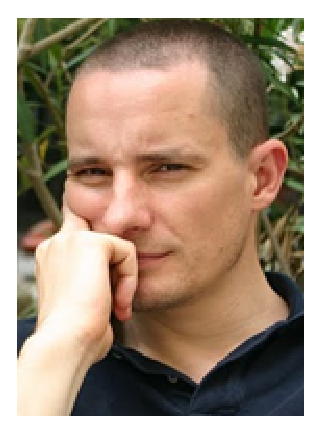
\includegraphics[width=19mm]{mikolaj}

$\exists \sigma$ (strategy for Eve),

$\forall \pi$ (paths), 

$\exists N \in \mathbb{N}$,

\end{minipage}
\hspace{0.5cm}
\begin{minipage}[b]{0.45\linewidth}
\centering
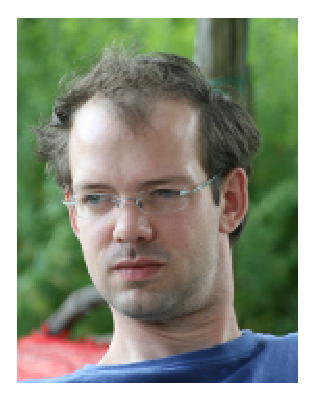
\includegraphics[width=20mm]{thomas}

$\exists \sigma$ (strategy for Eve),

$\exists N \in \mathbb{N}$,

$\forall \pi$ (paths),
\end{minipage}
\end{figure}
\begin{center}
$\pi$ satisfies parity
and each counter is bounded by $N$.
\end{center}

\pause
\begin{figure}[ht]
\begin{minipage}[b]{0.45\linewidth}
\centering

non-uniform

$(\mathrm{MSO} + \mathbb{U})$
\end{minipage}
\hspace{0.5cm}
\begin{minipage}[b]{0.45\linewidth}
\centering

uniform

$(\mathrm{cost}\ \mathrm{MSO})$
\end{minipage}
\end{figure}
\end{frame}


\begin{frame}{Why finite-memory strategies?}
Thomas Colcombet's habilitation:
\vskip1em

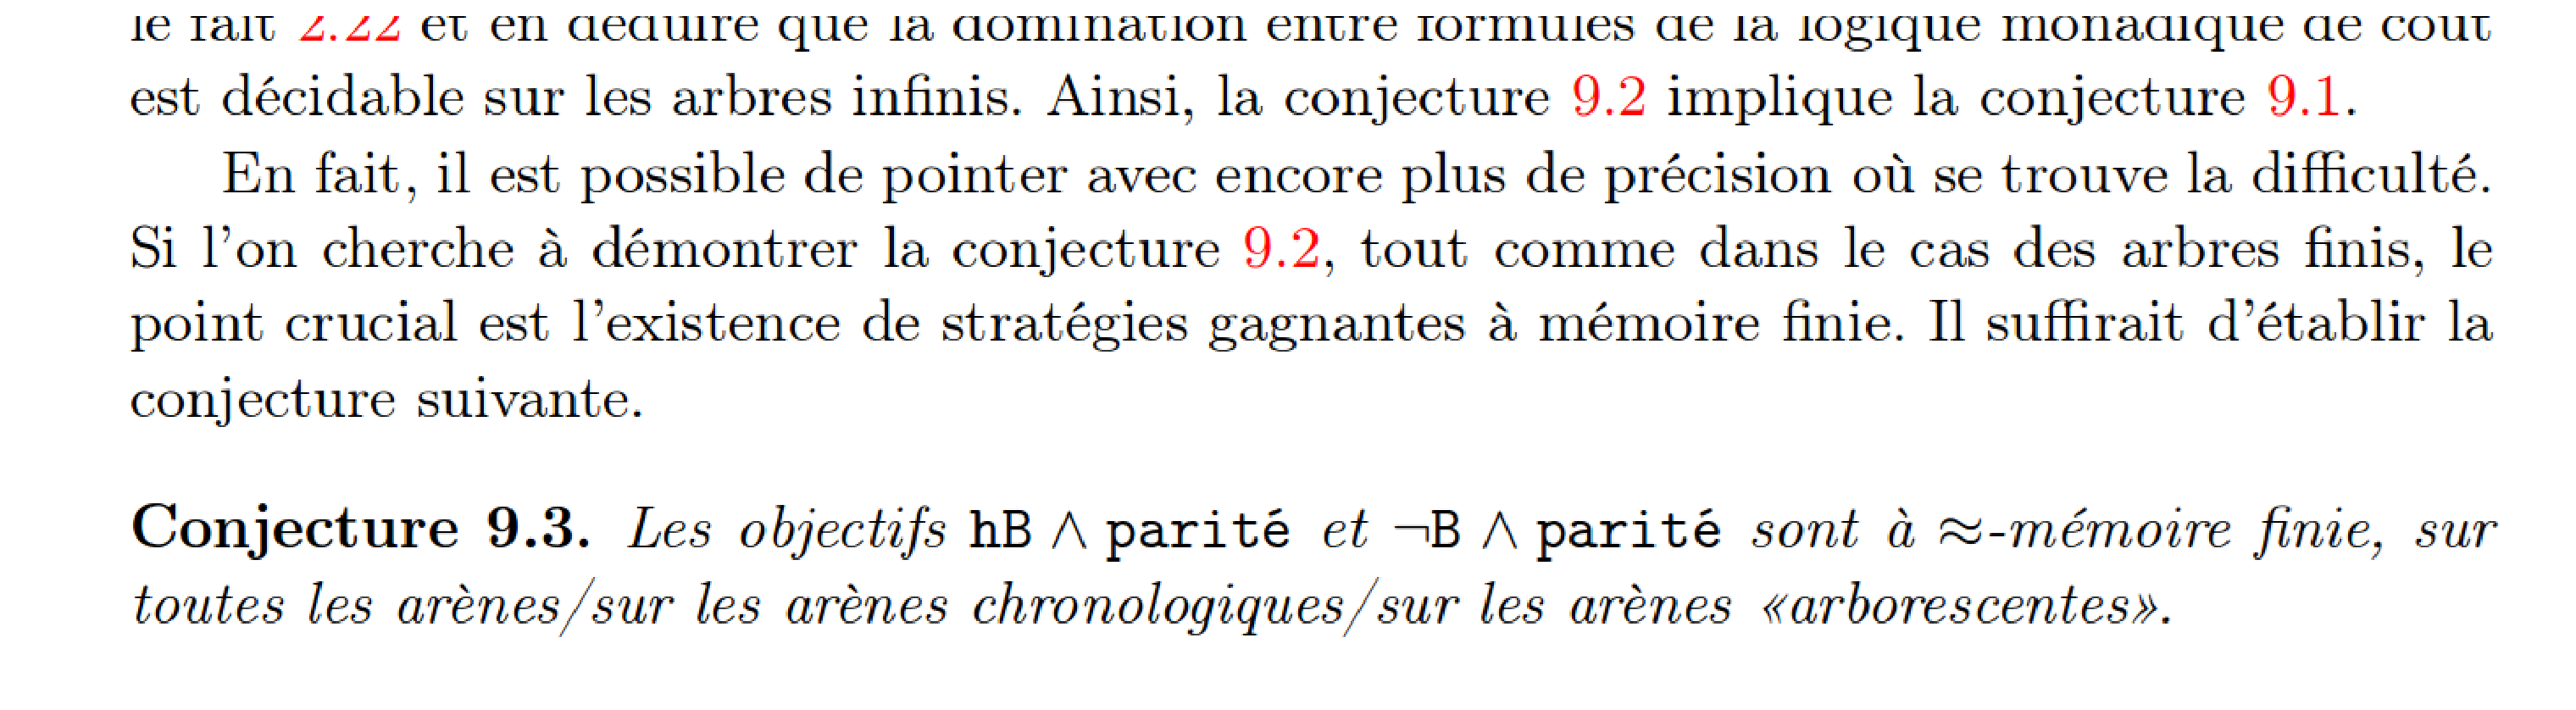
\includegraphics[width=100mm]{thomas_habilitation}

Existence of finite-memory strategies in (some) $\omega B$-games

$\Longrightarrow$ Decidability of cost MSO over infinite trees

$\Longrightarrow$ Decidability of the index of the non-deterministic Mostowski's hierarchy
(open for 40 years)!
\end{frame}


\begin{frame}{Contributions of this paper (1/2)}

Finitary conditions were introduced by Alur and Henzinger in 94,
and are a subclass of $\omega B$ conditions where
the counters and parity are not independent.
\vskip1em

\begin{theorem}[not in this talk]
Over general graphs, Eve has finite-memory winning strategies in finitary games.
\end{theorem}

\begin{theorem}[not in this talk]
Solving pushdown finitary games with stack boundedness condition is $\mathrm{EXPTIME}$-complete.
\end{theorem}
\end{frame}

\begin{frame}{Contributions of this paper (2/2)}
\begin{theorem}
Over pushdown graphs, the uniform and non-uniform quantifications are \textbf{almost} equivalent.
\end{theorem}

\begin{corollary}
Solving pushdown $\omega B$-games is decidable.
\end{corollary}
\end{frame}

\section{Equivalence for pushdown $\omega B$-games}

\begin{frame}{A first example}
\begin{figure}
\begin{center}
\begin{picture}(30,12)(0,0)
	\gasset{Nh=6,Nw=6}

	\node[Nmarks=i,iangle=-90](q)(0,5){}
	\rpnode[polyangle=45](p)(30,5)(4,4){}

	\drawedge[curvedepth=5](q,p){}
	\drawedge[curvedepth=5](p,q){$\begin{array}{c} \push(a) \\ r \end{array}$}

	\drawloop[loopangle=180](q){$\pop(a)$}
	\drawloop[loopangle=0](p){$\begin{array}{c} \pop(a) \\ i \end{array}$}
\end{picture}
\end{center}
\end{figure}
\vskip2em
Eve should maintain a low stack.
\end{frame}

\begin{frame}{Objective}
\begin{theorem}
For all pushdown games, the following are equivalent:
\begin{itemize}
	\item $\exists \sigma$ (strategy for Eve), $\forall \pi$ (paths), $\exists N \in \mathbb{N}$,\\
$\pi$ satisfies parity and each counter is bounded by $N$.
	\item $\exists \sigma$ (strategy for Eve), $\exists N \in \mathbb{N}$, $\forall \pi$ (paths),\\
$\pi$ satisfies parity and \textbf{eventually} each counter is bounded by $N$.
\end{itemize}
\end{theorem}

\pause

\begin{figure}[ht]
\begin{minipage}[b]{0.4\linewidth}
\centering
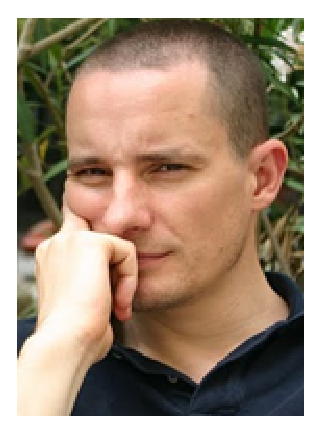
\includegraphics[width=19mm]{mikolaj}
\end{minipage}
\begin{minipage}[b]{0.4\linewidth}
\centering
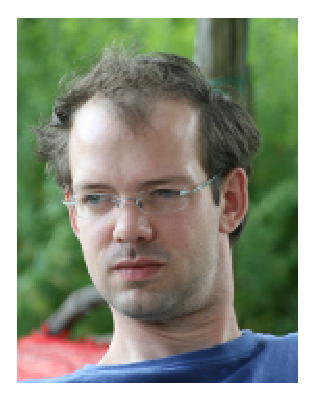
\includegraphics[width=20mm]{thomas}
\end{minipage}
\end{figure}
\end{frame}

\begin{frame}{Counter-example for the general case}
\begin{center}
\begin{figure}
\begin{picture}(65,40)(0,0)
	\rpnode[Nmarks=i,polyangle=45](v_0)(0,30)(4,3){}

	\rpnode[polyangle=45](v_1)(20,40)(4,3){}
	\rpnode[polyangle=45](v_2)(40,40)(4,3){}
	\put(45,39.5){\begin{Huge}$\ldots$\end{Huge}}
	\rpnode[polyangle=45](v_n)(60,40)(4,3){}
	\put(65,39.5){\begin{Huge}$\ldots$\end{Huge}}

	\rpnode[polyangle=45](u_11)(20,12)(4,3){}
	\rpnode[polyangle=45](u_12)(20,0)(4,3){}

	\rpnode[polyangle=45](u_21)(40,24)(4,3){}
	\rpnode[polyangle=45](u_22)(40,12)(4,3){}
	\rpnode[polyangle=45](u_23)(40,0)(4,3){}

	\rpnode[polyangle=45](u_n)(60,12)(4,3){}
	\put(65,11.5){\begin{Huge}$\ldots$\end{Huge}}

	\drawedge(v_0,v_1){}
	\drawedge(v_1,v_2){}
	\drawedge(v_1,u_11){}
	\drawedge(v_2,u_21){}
	\drawedge(v_n,u_n){}

	\drawedge[curvedepth=5](u_11,u_12){$i$}
	\drawedge[curvedepth=5](u_12,u_11){$r$}

	\drawedge[curvedepth=5](u_21,u_23){$i$}
	\drawedge[curvedepth=5](u_23,u_22){$i$}
	\drawedge[curvedepth=5](u_22,u_21){$r$}

	\drawloop[loopdiam=10,loopangle=-90,dash={3 1.5}{1.5}](u_n){$n$}
\end{picture}
\end{figure}
\end{center}

Eve wins but she does not know the bound!

\end{frame}

\subsection{The case of finite graphs}

\begin{frame}{A simple proof for the case of finite graphs}
Condition: parity and all counters are bounded.
\vskip1em

Define:
\begin{itemize}
	\item $\WE(N)$ the set of vertices where Eve wins for the bound $N$.
	\item $\WE$ the set of vertices where Eve wins for some (non-uniform) bound.
\end{itemize}

\pause
\begin{lemma}
\begin{enumerate}
	\item $\WE(0) \subseteq \WE(1) \subseteq \cdots \subseteq \WE(N) \subseteq \WE(N+1) \subseteq \cdots \subseteq \WE$.
\pause
	\item There exists $N$ such that $\WE(N) = \WE(N+1) = \cdots$.
\pause
	\item
For such $N$, Adam wins from $V \setminus \WE(N)$, hence $\WE = \WE(N)$.
\end{enumerate}
\end{lemma}
\end{frame}

\subsection{The case of pushdown graphs}

\begin{frame}{Another example}
\begin{figure}
\begin{center}
\begin{picture}(45,25)(0,0)
	\gasset{Nh=6,Nw=6}

	\rpnode[Nmarks=i,iangle=90,polyangle=45](q_0)(0,20)(4,4){}
	\rpnode[polyangle=45](q_1)(20,20)(4,4){}
	\rpnode[polyangle=45](q_2)(20,0)(4,4){}
	\rpnode[polyangle=45](q_3)(40,0)(4,4){}
	\rpnode[polyangle=45](q_4)(45,20)(4,4){}

	\drawloop[loopangle=180](q_0){$\push(a)$}
	\drawloop[loopangle=180](q_2){$\push(b)$}
	\drawloop[loopangle=0](q_3){$\begin{array}{c} \pop(b) \\ i \end{array}$}
	\drawloop[loopangle=0](q_4){}

	\drawedge(q_0,q_1){}
	\drawedge[ELside=r](q_1,q_2){$\pop(a)$}
	\drawedge(q_2,q_3){}
	\drawedge[curvedepth=-5](q_3,q_1){}
	\drawedge(q_1,q_4){}

\only<2>{\node[fillcolor=magenta,Nw=4,Nh=4](pebble)(0,20){}}
\only<3>{\node[fillcolor=magenta,Nw=4,Nh=4](pebble)(20,20){}}
\only<4>{\node[fillcolor=magenta,Nw=4,Nh=4](pebble)(20,0){}}
\only<5>{\node[fillcolor=magenta,Nw=4,Nh=4](pebble)(40,0){}}
\only<6>{\node[fillcolor=magenta,Nw=4,Nh=4](pebble)(20,20){}}
\only<7>{\node[fillcolor=magenta,Nw=4,Nh=4](pebble)(45,20){}}
\end{picture}
\end{center}
\end{figure}
\vskip1em
Adam may use the stack as ``credit''.
\end{frame}

\begin{frame}{Proof sketch}
Condition: parity and all counters are bounded.
\vskip1em

Define:
\begin{itemize}
	\item $\WE(N)$ the set of vertices where Eve wins for the bound $N$ \textbf{in the limit}.
	\item $\WE$ the set of vertices where Eve wins for some (non-uniform) bound.
\end{itemize}

\pause
\begin{proposition}
\begin{enumerate}
	\item $\WE(0) \subseteq \WE(1) \subseteq \cdots \subseteq \WE(N) \subseteq \WE(N+1) \subseteq \cdots \subseteq \WE$.
	\item There exists $N$ such that $\WE(N) = \WE(N+1) = \cdots$.
	\item For such $N$, Adam wins from $V \setminus \WE(N)$, hence $\WE = \WE(N)$.
\end{enumerate}
\end{proposition}
Why is 2. true?
\end{frame}

\begin{frame}{Regularity of the winning regions}

\begin{center}
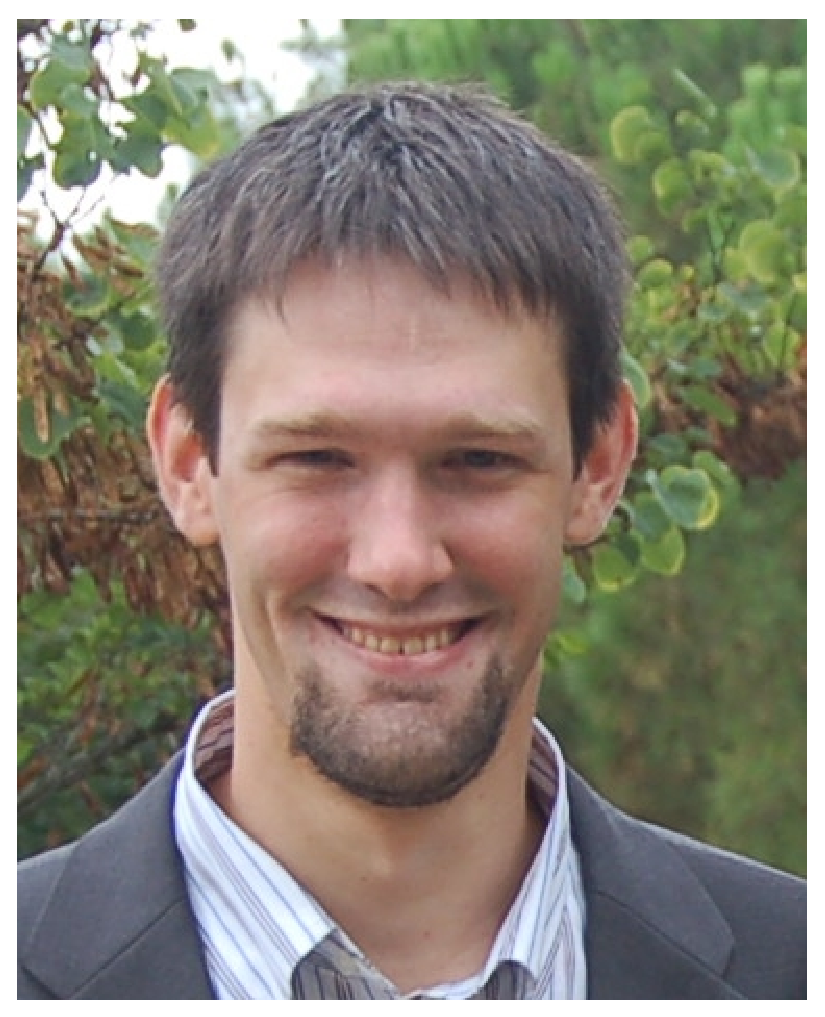
\includegraphics[width=20mm]{serre}
\end{center}

\begin{theorem}[derived from Serre]
For all $N$, $\WE(N)$ is a regular set of configurations, recognized by an alternating automaton
of size $|Q|$ (\textbf{independent of} $N$).
\end{theorem}
\end{frame}

\begin{frame}{Decidability}

\begin{theorem}
For all pushdown games, the following are equivalent:
\begin{itemize}
	\item $\exists \sigma$ (strategy for Eve), $\forall \pi$ (paths), $\exists N \in \mathbb{N}$,\\
$\pi$ satisfies parity and each counter is bounded by $N$.
	\item $\exists \sigma$ (strategy for Eve), $\exists N \in \mathbb{N}$, $\forall \pi$ (paths),\\
$\pi$ satisfies parity and \textbf{eventually} each counter is bounded by $N$.
\end{itemize}
\end{theorem}

\pause
\begin{corollary}
Determining the winner in a pushdown $\omega B$-game is decidable.
\end{corollary}

\pause
Remark: one can show that the collapse bound is doubly-exponential!
\end{frame}



\end{document}

